% ============================================================
%  MS-GARCH Likelihood Approximation Research Article
%  Journal-ready format (single-column, suitable for submission)
% ============================================================
\documentclass[12pt, a4paper]{article}

% ---- ENCODING & FONTS ----
\usepackage[utf8]{inputenc}
\usepackage[T1]{fontenc}
\usepackage{mathptmx}

% ---- PAGE LAYOUT ----
\usepackage[top=2.5cm, bottom=2.5cm, left=3cm, right=3cm]{geometry}
\usepackage{setspace}
\onehalfspacing

% ---- CORE PACKAGES ----
\usepackage{amsmath, amssymb}
\usepackage{graphicx}
\graphicspath{{../results/plots/}}
\usepackage{subcaption}
\usepackage{array, booktabs, multirow, longtable}
\usepackage{adjustbox}
\usepackage{float}
\usepackage{caption}
\captionsetup{font=small, labelfont=bf}
\usepackage{rotating}
\usepackage{pdflscape}

% ---- BIBLIOGRAPHY ----
\usepackage[authoryear, round, sort]{natbib}
\bibliographystyle{apalike}

% ---- LINKS ----
\usepackage[hidelinks, colorlinks=false]{hyperref}

% ---- HEADER / FOOTER ----
\setlength{\headheight}{14pt}
\usepackage{fancyhdr}
\pagestyle{fancy}
\fancyhf{}
\fancyhead[L]{\small\textit{Ogundairo \& Ojo}}
\fancyhead[R]{\small\textit{MS-GARCH Likelihood Approximation}}
\fancyfoot[C]{\thepage}
\renewcommand{\headrulewidth}{0.4pt}

% ---- PARAGRAPH STYLE ----
\setlength{\parindent}{1.5em}
\setlength{\parskip}{4pt}

% ---- SECTION FORMAT ----
\usepackage{titlesec}
\titleformat{\section}{\normalfont\large\bfseries}{\thesection.}{0.8em}{}
\titleformat{\subsection}{\normalfont\normalsize\bfseries}{\thesubsection.}{0.6em}{}
\titlespacing*{\section}{0pt}{12pt}{6pt}
\titlespacing*{\subsection}{0pt}{8pt}{4pt}

% ---- ABSTRACT BOX ----
\usepackage{mdframed}
\mdfsetup{linewidth=0.5pt, innertopmargin=8pt, innerbottommargin=8pt,
          innerleftmargin=10pt, innerrightmargin=10pt}

% ---- LISTS ----
\usepackage{enumitem}

% ---- MISC ----
\usepackage{url}
\usepackage{microtype}

% ===========================================================
%  DOCUMENT START
% ===========================================================
\begin{document}

% ---- TITLE BLOCK ----
\begin{center}
{\LARGE \bfseries Impact of Likelihood Approximation Choices on the Performance of Markov-Switching GARCH Models: Evidence from Thirty Global Financial Assets}

\vspace{1.2em}

{\large
Joshua Ogundairo\textsuperscript{a,*} \quad and \quad Oluwadare O. Ojo\textsuperscript{a}
}

\vspace{0.6em}

{\small
\textsuperscript{a}Department of Statistics, Federal University of Technology, Akure (FUTA), Nigeria\\[2pt]
\textsuperscript{*}Corresponding author. Email: \href{mailto:ogundairosta154470@futa.edu.ng}{ogundairosta154470@futa.edu.ng}\\
O. O. Ojo email: \href{mailto:ojooo@futa.edu.ng}{ojooo@futa.edu.ng}
}

\vspace{1em}
{\small Date: June 2026}
\end{center}

\vspace{1em}
\hrule
\vspace{0.5em}

% ---- ABSTRACT ----
\begin{mdframed}
\singlespacing\small
\noindent\textbf{Abstract}

\noindent
This study evaluates the comparative performance of four likelihood approximation methods for Markov-Switching GARCH(1,1) models across thirty financial assets spanning five market archetypes: equities, bonds, cryptocurrencies, derivatives, and foreign exchange. The approximation methods evaluated are Gray's moment-matching collapsing procedure, the Plug-in approximation, five-point Gauss-Hermite Quadrature, and a Particle Filter employing sequential importance resampling with 1,000 particles. Models were estimated under both baseline (internal volatility dynamics only) and exogenous (cross-market spillover conditioning) specifications, yielding 220 experimental cases. Assets are classified into four excess-kurtosis cohorts — low ($K < 10$), medium ($10 \le K < 20$), high ($20 \le K < 50$), and extreme ($K \ge 50$) — to assess how distributional tail behaviour moderates approximation performance. The Plug-in method dominated log-likelihood maximisation across all kurtosis classes and market archetypes, often surpassing Gray's collapsing and Quadrature by more than 2{,}000 log-likelihood units for equity-index futures. Gray and Quadrature provided superior convergence reliability for cryptocurrency assets under exogenous conditioning. The Particle Filter achieved the broadest convergence coverage but was universally the worst likelihood optimiser, underperforming analytical alternatives by two to four thousand units across all asset classes and exhibiting parameter trapping near initialisation values. The CBOE Volatility Index (\^{}VIX) was the sole instrument for which all analytical methods failed to converge in every specification, representing a fundamental estimation boundary for the adopted framework. Exogenous conditioning produced selective rather than uniform improvements, with bond and equity markets benefiting most. A kurtosis-informed method-selection framework is proposed for practitioners.

\vspace{0.5em}
\noindent\textbf{Keywords:} Markov-switching GARCH; likelihood approximation; particle filter; Gaussian quadrature; kurtosis; regime switching; volatility modelling

\noindent\textbf{JEL Classification:} C13; C63; G12; G17
\end{mdframed}
\vspace{1em}
\hrule
\vspace{1.5em}

% ===========================================================
\section{Introduction}
% ===========================================================

Regime-switching models have become fundamental tools in financial econometrics for capturing the discrete alternation between qualitatively distinct market states that characterises asset return dynamics. Among these, the Markov-Switching Generalised Autoregressive Conditional Heteroskedasticity (MS-GARCH) model represents a particularly sophisticated framework, combining the discrete regime-transition structure of Hidden Markov Models with the continuous volatility clustering dynamics of GARCH processes \citep{Hamilton1989, Haas2004}. The appeal of this formulation lies in its ability to simultaneously address two empirically important features of financial returns: within-regime volatility persistence, and abrupt structural shifts between fundamentally different market states. Empirical applications have demonstrated the value of this framework across numerous asset classes, with MS-GARCH models frequently outperforming single-regime alternatives in volatility forecasting, risk measurement, and regime identification \citep{Klaassen2002, Ardia2018, Guidolin2007}.

Despite these advantages, the practical estimation of MS-GARCH models confronts a fundamental computational barrier that has received insufficient systematic attention in the methodological literature. The challenge arises from the path-dependent nature of the GARCH volatility recursion interacting with the presence of unobserved regime transitions. Because the conditional variance at any time point depends on past variances, which themselves depend on the sequence of regimes prevailing when they were formed, exact likelihood evaluation requires summing over all $2^T$ possible regime histories for a sample of length $T$. For even modest sample sizes, this number grows far beyond any conceivable computational capacity \citep{Gray1996, Haas2004, Bauwens2010}. Researchers have consequently developed several approximation strategies to render estimation tractable: Gray's moment-matching collapsing procedure \citep{Gray1996}, plug-in approximations that substitute filtered probability estimates for regime uncertainty \citep{Klaassen2002, Durbin2012}, quadrature-based numerical integration methods \citep{Tanizaki1996}, and particle filtering via sequential Monte Carlo techniques \citep{Doucet2009, Pitt1999}.

Each approximation strategy introduces errors of distinct types and magnitudes. Gray's procedure and quadrature methods introduce deterministic error whose accuracy improves with finer discretisation but at increasing computational cost \citep{Haas2004, Augustyniak2014}. Plug-in methods generate a different error by treating uncertain regime assignments as known quantities, potentially inducing bias through the omission of regime uncertainty \citep{Durbin2012}. Particle filters introduce Monte Carlo variability whose magnitude depends on population size and resampling choices, and are susceptible to particle degeneracy and impoverishment \citep{Doucet2001, Pitt1999}. Notwithstanding these fundamental differences, the applied MS-GARCH literature provides remarkably limited guidance for approximation method selection. Most studies adopt whichever method is most convenient — frequently Gray's procedure by default — without evaluating whether results would remain robust under alternative computational approaches \citep{Augustyniak2014, Catania2019, Ardia2019}.

This gap in systematic comparative evidence carries practical consequences. When different research teams apply different approximation methods to similar research questions, divergent findings emerge that cannot be attributed unambiguously to genuine economic heterogeneity rather than computational artifacts. Financial institutions employing MS-GARCH models for risk management, Value-at-Risk estimation, or portfolio allocation similarly face uncertainty about whether their choice of approximation method materially affects outputs \citep{Ardia2018, Guidolin2007}. The few existing comparative studies rely predominantly on simulation experiments with data from known processes, leaving the relative performance of approximation methods on real financial data — with their heavy tails, asymmetric responses, and unknown true regimes — largely unexplored \citep{Augustyniak2014}.

This paper addresses these gaps through a controlled empirical investigation that holds the MS-GARCH(1,1) model specification constant while systematically varying the likelihood approximation method across thirty financial assets drawn from five distinct market archetypes: equities, bonds, cryptocurrencies, derivatives, and foreign exchange. Both baseline (internal dynamics) and exogenous (cross-market spillover) specifications are estimated for each asset, yielding 220 experimental cases. Assets are further classified into four kurtosis cohorts to assess whether distributional tail behaviour mediates approximation performance. The findings provide the first large-scale, multi-market comparative assessment of likelihood approximation methods for MS-GARCH models under real financial data conditions, offering evidence-based guidance for method selection. The remainder of the paper proceeds as follows: Section~\ref{sec:methodology} details the methodology; Section~\ref{sec:results} presents market-level findings; Section~\ref{sec:discussion} develops the kurtosis-based discussion; and Section~\ref{sec:conclusion} concludes.

% ===========================================================
\section{Methodology}
\label{sec:methodology}
% ===========================================================

\subsection{Theoretical Background}

The empirical analysis employs a two-regime MS-GARCH(1,1) model in which observed returns are generated by a latent Markov chain $\{S_t\}_{t=1}^T$, $S_t \in \{1, 2\}$, evolving with constant transition probabilities:
\begin{equation}
p_{jk} = \Pr(S_t = k \mid S_{t-1} = j), \quad j, k \in \{1, 2\},
\end{equation}
collected in the transition matrix $P = (p_{jk})$ with $\sum_k p_{jk} = 1$. Conditional on the regime, returns follow:
\begin{equation}
y_{i,t} = \mu_{i,S_t} + \sigma_{i,t}(S_t)\,\varepsilon_{i,t}, \quad \varepsilon_{i,t} \sim \mathcal{N}(0,1),
\end{equation}
with regime-dependent conditional mean $\mu_{i,k} = c_{i,k} + \gamma_{i,k}\,x_t$ (exogenous specification) or $\mu_{i,k} = c_{i,k}$ (baseline), where $x_t$ is the log-return of the market pivot asset. The conditional variance follows a GARCH(1,1) process within each regime:
\begin{equation}
\sigma_{i,t}^2(k) = \omega_{i,k} + \alpha_{i,k}\,y_{i,t-1}^2 + \beta_{i,k}\,\sigma_{i,t-1}^2,
\end{equation}
with $\omega_{i,k} > 0$, $\alpha_{i,k} \ge 0$, $\beta_{i,k} \ge 0$, and $\alpha_{i,k} + \beta_{i,k} < 1$ for within-regime stationarity. The full parameter vector is $\Psi_i = \{c_{i,1}, c_{i,2}, \gamma_{i,1}, \gamma_{i,2}, \omega_{i,1}, \omega_{i,2}, \alpha_{i,1}, \alpha_{i,2}, \beta_{i,1}, \beta_{i,2}, p_{11}, p_{22}\}$, comprising twelve parameters. Exact maximum likelihood evaluation requires integrating over all $2^T$ regime sequences through the recursion:
\begin{equation}
L(\Psi_i) = \sum_{S_1=1}^{2}\cdots\sum_{S_T=1}^{2} \pi_{S_1}\prod_{t=2}^T p_{S_{t-1},S_t}\prod_{t=1}^T f(y_{i,t}\mid S_t, \mathcal{F}_{t-1};\Psi_i),
\end{equation}
which is computationally intractable due to the path-dependence of the GARCH variance recursion.

Gray's Collapsing Procedure addresses path-dependence by moment-matching the expanding variance distribution onto two representative values at each time step. At time $t$, the approximate conditional variance for regime $k$ is \citep{Gray1996}:
\begin{equation}
\tilde{\sigma}_{i,t}^2(k) = \omega_{i,k} + \alpha_{i,k}\,y_{i,t-1}^2 + \beta_{i,k}\,\bar{\sigma}_{i,t-1}^2(k),
\end{equation}
where $\bar{\sigma}_{i,t-1}^2(k) = \sum_j \Pr(S_{t-1}=j|S_t=k)\,\tilde{\sigma}_{i,t-1}^2(j)$ is the probability-weighted average from the previous period.

Gaussian Quadrature maintains $N$ quadrature nodes $\{\nu_n\}$ and weights $\{w_n\}$ to approximate expectations under the variance distribution, here using a five-point Gauss-Hermite scheme ($N=5$). The algorithm maintains $N \times 2$ distinct variance paths and computes likelihood contributions by summing over these paths \citep{Tanizaki1996, Monfort2015}.

Plug-In Approximation replaces integration over regime uncertainty with point estimates based on filtered probabilities. The plug-in variance is \citep{Klaassen2002}:
\begin{equation}
\hat{\sigma}_{i,t}^2 = \sum_{k=1}^{2}\Pr(S_t=k|\mathcal{F}_{t-1})\,\sigma_{i,t}^2(k),
\end{equation}
with $\sigma_{i,t}^2(k) = \omega_{i,k} + \alpha_{i,k}\,y_{i,t-1}^2 + \beta_{i,k}\,\hat{\sigma}_{i,t-1}^2$.

Particle Filter represents the variance path distribution through $N_p = 1{,}000$ weighted random samples (particles) propagated forward via sequential importance resampling (SIR) \citep{Doucet2009, Pitt1999}. Each particle $n$ carries a regime sequence and corresponding variance path:
\begin{equation}
\sigma_{i,t}^{2(n)} = \omega_{i,S_t^{(n)}} + \alpha_{i,S_t^{(n)}}\,y_{i,t-1}^2 + \beta_{i,S_t^{(n)}}\,\sigma_{i,t-1}^{2(n)}.
\end{equation}
A fixed random seed ensures reproducibility across all 220 runs.

\subsection{Data and Sources}

Daily return series are sourced via the \texttt{yfinance} Python library for thirty financial assets over September 2015 through August 2025, a ten-year horizon encompassing multiple market cycles including the COVID-19 shock and subsequent inflationary episode. The corpus is stratified across five market archetypes, each comprising five target assets and one pivot asset serving as the exogenous conditioning variable:
\begin{itemize}[noitemsep, topsep=3pt, leftmargin=1.5em]
  \item Equities: FTSE, N225, IXIC, EEM, VTV; pivot = GSPC
  \item Bonds: IEI, TLT, BNDX, LQD, HYG; pivot = TNX
  \item Cryptocurrencies: ETH-USD, LTC-USD, XRP-USD, DOGE-USD, NMC-USD; pivot = BTC-USD
  \item Derivatives: ES=F, NQ=F, VIX, GC=F, CL=F; pivot = BTC=F
  \item Forex: GBPUSD=X, JPY=X, AUDUSD=X, CHF=X, EURGBP=X; pivot = EURUSD=X
\end{itemize}

All price series are transformed to continuously compounded percentage returns: $y_{i,t} = 100 \times \log(P_{i,t}/P_{i,t-1})$. All series pass Augmented Dickey-Fuller stationarity tests and Engle's ARCH-LM tests for conditional heteroskedasticity ($p < 0.001$ throughout), confirming the suitability of GARCH-type modelling. Table~\ref{tab:descriptive} summarises the distributional properties of all thirty assets.

\subsection{Experimental Setup and Specifications}

For each of the thirty assets, two model specifications are estimated with each of the four approximation methods, yielding 220 experimental cases in total. The \textit{baseline} specification ($\gamma_{i,k} = 0$) captures internal regime-dependent volatility dynamics without external conditioning. The \textit{exogenous} specification incorporates the market pivot ($\gamma_{i,k} \ne 0$) to capture cross-market spillovers. Pivot assets are estimated under the baseline specification only. Estimation employs the L-BFGS-B algorithm via \texttt{scipy.optimize} with box constraints enforcing parameter validity ($\omega > 0$, $\alpha + \beta < 1$, $0 < p_{ii} < 1$), implemented in a custom C++ engine interfaced with Python via Cython for computational efficiency. A penalty mechanism redirects the optimiser from infeasible parameter regions.

The kurtosis-based classification of assets, which informed the evaluation framework, emerged from the preliminary distributional analysis. Assets with excess kurtosis $K < 10$ (low kurtosis) include stable Forex pairs and short-duration bond instruments. Medium-kurtosis assets ($10 \le K < 20$) comprise equity indices, several cryptocurrencies, and the VIX. High-kurtosis assets ($20 \le K < 50$) include equity ETFs, corporate bonds, energy derivatives, and the 10-year Treasury yield. Extreme-kurtosis assets ($K \ge 50$) comprise DOGE-USD ($K = 98.51$) and EURGBP=X ($K = 248.50$).

\subsection{Evaluation Metrics}

Approximation performance is assessed through a multidimensional framework: (i) Log-Likelihood (LogLik) — the primary optimisation criterion, measuring goodness-of-fit; (ii) Akaike Information Criterion (AIC $= -2\,\text{LogLik} + 2k$, $k = 12$) — penalised fit for parsimony; (iii) Convergence status (binary indicator, TRUE when gradient norm satisfies L-BFGS-B stopping criterion) — a measure of numerical stability; and (iv) Regime persistence ($p_{11}$, $p_{22}$) — characterising the stability of the identified low- and high-volatility regimes. A method is considered dominant if it achieves the highest LogLik for a given asset and specification, regardless of convergence status. Convergence-adjusted dominance requires the highest LogLik among converged solutions.

\begin{table*}[ht]
\centering
\caption{Descriptive Statistics of Daily Log-Returns (\%)}
\label{tab:descriptive}
\resizebox{\linewidth}{!}{%
\begin{tabular}{llrrrrccc}
\toprule
\textbf{Asset} & \textbf{Market} & \textbf{Mean} & \textbf{StdDev} & \textbf{Skew} & \textbf{Excess Kurt.} & \textbf{Kurt.\ Class} & \textbf{ADF ($p$)} & \textbf{ARCH-LM ($p$)} \\
\midrule
\multicolumn{9}{l}{\textit{Bond Market}} \\
IEI   & Bond     & 0.0044 & 0.2205 & 0.3795  & 5.68  & Low    & 0.0000  & 5.53e-45  \\
TLT   & Bond     & -0.0071 & 0.8337 & 0.0705  & 8.12  & Low    & 2.17e-20 & 1.19e-139 \\
BNDX  & Bond     & 0.0045 & 0.2273 & -0.6025 & 11.68 & Medium & 0.0000  & 1.23e-96  \\
LQD   & Bond     & 0.0062 & 0.4979 & 0.3778  & 36.95 & High   & 9.68e-24 & 6.18e-190 \\
HYG   & Bond     & 0.0128 & 0.4695 & -0.0644 & 37.30 & High   & 1.69e-20 & 1.29e-117 \\
TNX   & Bond     & 0.0251 & 2.7052 & 0.3490  & 47.73 & High   & 1.46e-14 & 1.69e-249 \\ \midrule
\multicolumn{9}{l}{\textit{Cryptocurrency}} \\
ETH-USD  & Crypto & 0.0625 & 4.5557 & -0.8818 & 10.91 & Medium & 8.55e-29 & 1.45e-13 \\
LTC-USD  & Crypto & -0.0404 & 4.8588 & -0.5167 & 7.94  & Low    & 0.0000  & 1.81e-18 \\
XRP-USD  & Crypto & 0.0470 & 5.5694 & 0.6839  & 17.33 & Medium & 0.0000  & 2.69e-20 \\
DOGE-USD & Crypto & 0.1266 & 6.8135 & 4.7529  & 98.51 & Extreme& 6.99e-16 & 4.04e-10 \\
NMC-USD  & Crypto & -0.0455 & 7.8798 & -0.9870 & 29.31 & High   & 6.97e-19 & 6.71e-38 \\
BTC-USD  & Crypto & 0.0635 & 3.5104 & -0.9417 & 13.89 & Medium & 0.0000  & 1.95e-10 \\ \midrule
\multicolumn{9}{l}{\textit{Derivatives}} \\
ES=F  & Derivative & 0.0329 & 1.0404 & -0.7946 & 20.95 & High   & 3.68e-20 & 9.67e-138 \\
NQ=F  & Derivative & 0.0470 & 1.2778 & -0.3442 & 10.58 & Medium & 1.39e-17 & 7.92e-80  \\
VIX   & Derivative & 0.0108 & 6.7940 & 1.7173  & 14.28 & Medium & 0.0000  & 2.13e-16  \\
GC=F  & Derivative & 0.0363 & 0.8025 & -0.2476 & 6.58  & Low    & 0.0000  & 3.26e-33  \\
CL=F  & Derivative & 0.0254 & 2.4723 & 0.0479  & 39.31 & High   & 6.76e-17 & 2.33e-95  \\
BTC=F & Derivative & 0.0628 & 3.5341 & -0.2230 & 8.21  & Low    & 0.0000  & 3.20e-10  \\ \midrule
\multicolumn{9}{l}{\textit{Equities}} \\
FTSE  & Equity & 0.0080 & 0.8322 & -1.3901 & 25.19 & High   & 2.12e-25 & 5.11e-121 \\
N225  & Equity & 0.0233 & 1.0739 & -0.5317 & 17.57 & Medium & 0.0000  & 8.42e-107 \\
IXIC  & Equity & 0.0415 & 1.2542 & -0.4579 & 12.87 & Medium & 1.29e-25 & 1.25e-92  \\
GSPC  & Equity & 0.0329 & 1.0377 & -0.7358 & 22.64 & High   & 6.07e-20 & 8.80e-138 \\
EEM   & Equity & 0.0103 & 1.1082 & -0.9329 & 16.92 & Medium & 1.31e-28 & 1.86e-110 \\
VTV   & Equity & 0.0279 & 0.9566 & -0.9430 & 27.39 & High   & 3.09e-20 & 1.95e-182 \\ \midrule
\multicolumn{9}{l}{\textit{Forex}} \\
GBPUSD=X & Forex & 0.0006 & 0.4688 & -0.2666 & 8.04  & Low    & 3.94e-30 & 5.42e-41  \\
JPY=X    & Forex & 0.0095 & 0.4643 & -0.4158 & 6.56  & Low    & 0.0000  & 1.27e-20  \\
AUDUSD=X & Forex & -0.0056 & 0.5424 & -0.3614 & 6.83  & Low    & 0.0000  & 3.88e-22  \\
CHF=X    & Forex & -0.0075 & 0.3975 & -0.7058 & 8.14  & Low    & 0.0000  & 7.51e-22  \\
EURGBP=X & Forex & -0.0009 & 0.4546 & 0.2235  & 248.50& Extreme& 0.0000  & 1.48e-240 \\
EURUSD=X & Forex & -0.0002 & 0.3865 & -0.0128 & 4.49  & Low    & 0.0000  & 6.92e-19  \\
\bottomrule
\end{tabular}
}% end resizebox
\smallskip\\
\footnotesize Note: Mean and StdDev are in percentage (\%). Excess Kurtosis is relative to the normal distribution ($K=0$). All ADF and ARCH-LM $p$-values are $< 0.001$, confirming stationarity and ARCH effects throughout.
\end{table*}

% ===========================================================
\section{Results}
\label{sec:results}
% ===========================================================

Figure~\ref{fig:returns} illustrates the daily return profiles of all thirty assets across the five market archetypes. The wide dispersion in return volatility — ranging from the subdued fluctuations of short-duration bond ETFs to the violent, spike-dominated dynamics of cryptocurrencies and the VIX — underscores the importance of subjecting the approximation methods to a genuinely diverse empirical environment. Figure~\ref{fig:comparative} summarises the comparative log-likelihood performance across methods, providing a visual overview of the results described in the paragraphs below. Full parameter estimates for all 220 models are provided in a companion reference document (see supplementary file: \texttt{ms\_garch\_full\_models.pdf}).

\begin{figure}[!t]
\centering
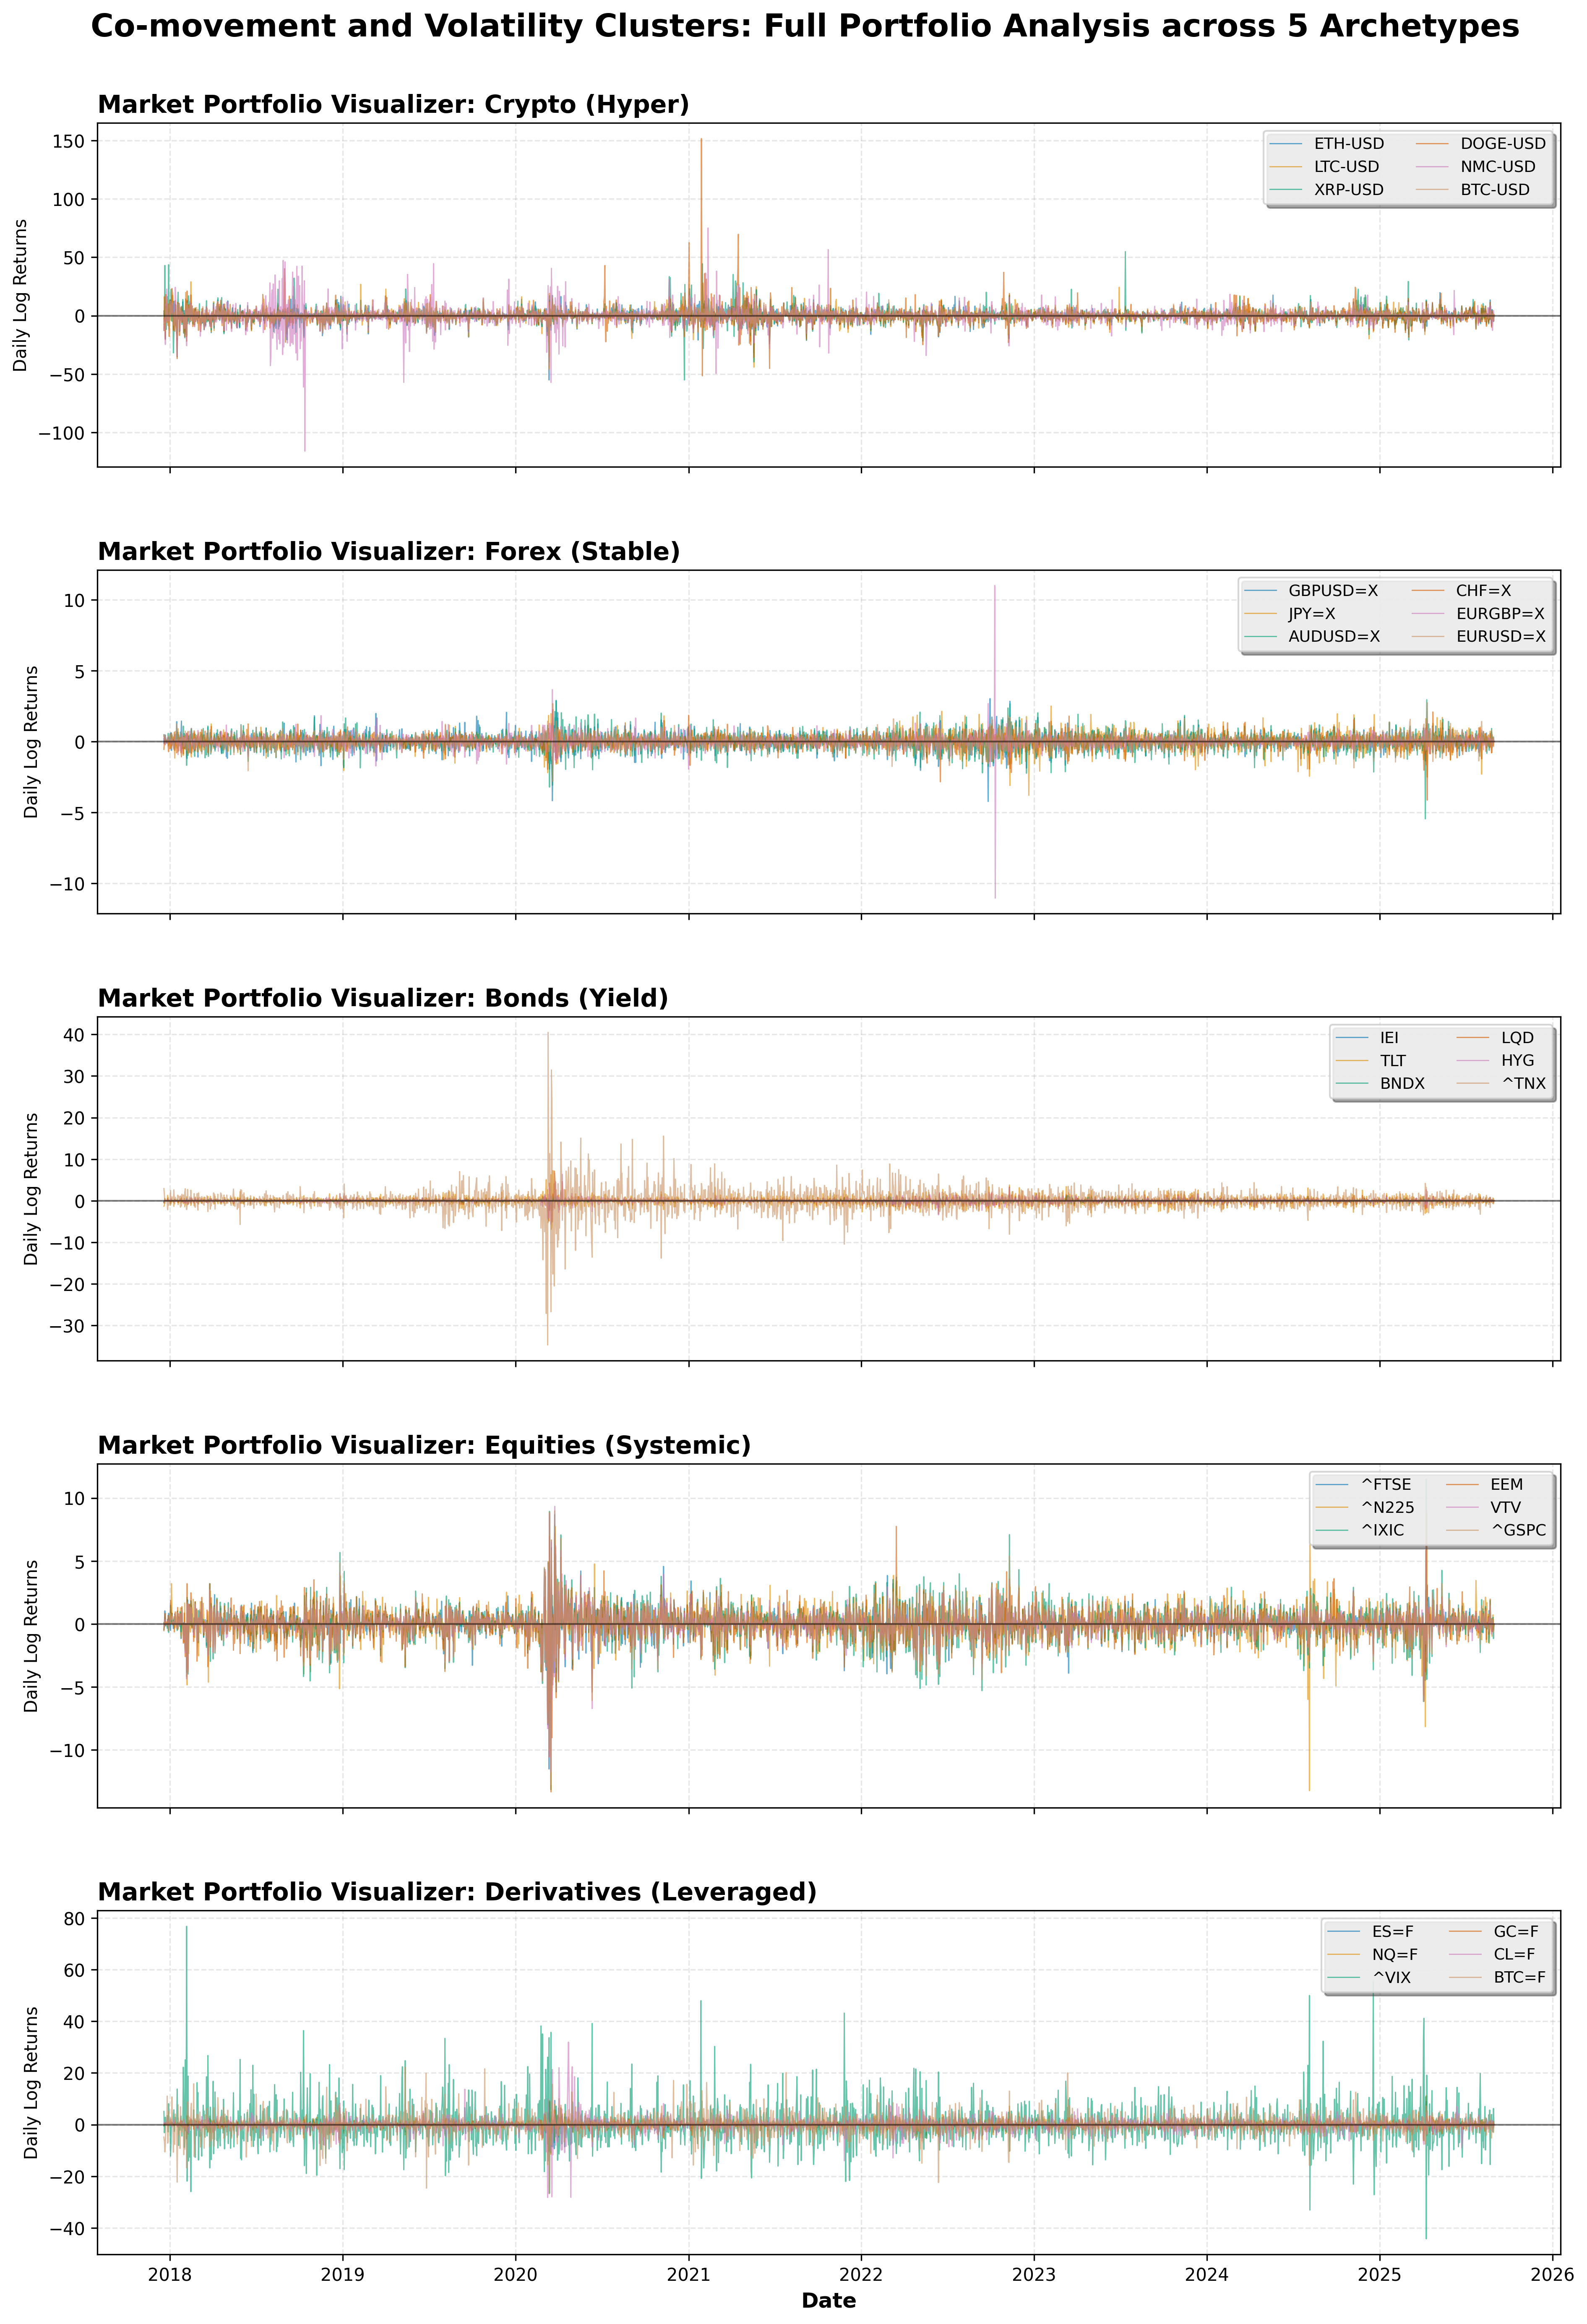
\includegraphics[width=\textwidth]{Full_Portfolio_Market_Visualization_5_Panes.png}
\caption{Daily Log-Return Series for All Thirty Assets, Stratified by Market Archetype (Sep 2015 -- Aug 2025). Shaded bands indicate the COVID-19 shock period (Mar--Apr 2020).}
\label{fig:returns}
\end{figure}

Cryptocurrency Market.
The cryptocurrency market constituted the most challenging estimation environment, reflecting the extreme excess kurtosis documented in Table~\ref{tab:descriptive}. In the baseline specification, the Plug-in method achieved the best log-likelihood for four of the six assets — ETH-USD ($-8{,}073.57$), LTC-USD ($-8{,}269.21$), DOGE-USD ($-8{,}613.45$), and BTC-USD ($-7{,}232.32$) — while Quadrature delivered the best fit for XRP-USD ($-8{,}514.52$). For NMC-USD, Quadrature ($-9{,}121.91$) marginally outperformed Gray ($-9{,}126.19$), with Plug-in inferior at $-9{,}326.54$. However, Plug-in frequently failed the formal convergence criterion despite reaching superior likelihood values, a pattern consistent with rough likelihood surfaces generated by high-kurtosis return series. Gray's method converged for BTC-USD and ETH-USD but achieved consistently lower log-likelihoods than Plug-in. The Particle Filter, though achieving convergence for most assets, was universally the weakest estimator with log-likelihoods ranging from $-7{,}854$ (BTC-USD) to $-10{,}526$ (NMC-USD), far below the analytical alternatives, and its parameter estimates exhibited degeneracy near initialisation values ($\omega \approx 0.30$, $\alpha \approx 0.05$, $\beta \approx 0.85$, $p_{11} \approx 0.95$, $p_{22} \approx 0.80$). In the exogenous specification conditioned on BTC-USD, Gray and Quadrature emerged as the most reliable combination. Both methods jointly achieved the best converged log-likelihoods for ETH-USD ($-8{,}072.60$ and $-8{,}072.25$, respectively) and LTC-USD ($-8{,}292.09$ and $-8{,}291.69$), with Plug-in producing inferior values and failing convergence more frequently under the exogenous configuration. The Particle Filter remained invariant to the pivot specification, continuing to produce near-initialisation persistence estimates in both states. Near-unit persistence values ($> 0.90$) across most crypto assets under the analytical methods confirmed the well-documented volatility persistence of digital asset returns, while exogenous conditioning with BTC-USD produced modest rather than dramatic changes in regime dynamics, indicating that intra-market spillovers are not the dominant driver of within-sample volatility clustering in cryptocurrencies.

Foreign Exchange (Forex) Market.
The Forex market produced a consistent pattern of Plug-in superiority in likelihood maximisation across both specifications. In the baseline, Plug-in achieved the highest log-likelihood for every Forex asset: GBPUSD=X ($63.64$), JPY=X ($71.36$), AUDUSD=X ($-376.14$), CHF=X ($372.12$), EURGBP=X ($557.11$), and EURUSD=X ($399.99$). Gray's method ranked second in most cases, with Quadrature third. The Particle Filter exhibited the most striking underperformance of any market, with log-likelihoods ranging from approximately $-1{,}879$ to $-2{,}384$ — deficiencies of two to four thousand log-likelihood units relative to the analytical methods — despite achieving formal convergence for most assets. The transition from baseline to exogenous specifications conditioned on EURUSD=X produced negligible changes in log-likelihood across all currency pairs, with representative shifts of less than two log-likelihood units (e.g., CHF=X Gray: $302.30 \to 303.39$; Plug-in: $372.12 \to 372.35$), confirming that Forex volatility regimes are predominantly determined by idiosyncratic currency dynamics rather than cross-currency spillovers from the Euro-Dollar benchmark. Convergence was broadly stable for the analytical methods in both specifications, with the notable exception of JPY=X, where Gray, Plug-in, and Quadrature all registered non-convergence in the exogenous configuration, suggesting that the EURUSD=X factor marginally destabilised the Yen-Dollar likelihood surface. The analytical methods identified a two-state structure with a highly persistent primary regime ($p_{ii} > 0.95$) and a near-transient secondary regime ($p_{ii} \approx 0.0002$), reflecting the low-volatility environment characterising major developed-market currency pairs over the study decade.

Equity Market.
Equity results revealed a consistent and substantial advantage for the Plug-in method in likelihood maximisation. In the baseline specification, Plug-in achieved the best log-likelihood for FTSE ($-753.01$), N225 ($-1{,}183.10$), IXIC ($-1{,}647.97$), EEM ($-1{,}451.69$), and VTV ($-835.80$). The magnitude of the Plug-in advantage over Gray and Quadrature was particularly striking for IXIC and EEM: the Gray model for IXIC reached only $-4{,}070.86$ while Plug-in achieved $-1{,}647.97$ — a gap of over 2{,}400 log-likelihood units — and for EEM, Gray reached $-3{,}672.50$ (non-converged) against Plug-in's $-1{,}451.69$. The GSPC pivot itself showed a different pattern: Gray was the only converged analytical method in the baseline ($-3{,}333.75$), while Plug-in ($-1{,}054.82$) and Quadrature ($-1{,}414.35$) reached better likelihoods but failed formal convergence. In the exogenous configuration conditioned on GSPC, Plug-in retained its dominant position with consistent improvements for most assets: FTSE improved from $-753.01$ to $-726.36$; N225 improved from $-1{,}183.10$ to $-958.26$. Gray's method suffered markedly from the introduction of the exogenous pivot: for N225, Gray deteriorated from $-1{,}523.48$ (converged) in the baseline to $-3{,}164.01$ (non-converged) in the exogenous model, indicating that the additional gamma parameters interacted adversely with the moment-matching procedure's stability for several equity assets. The Particle Filter was the weakest performer across all equity assets in both specifications, with log-likelihoods consistently two to four thousand units below Plug-in and parameter estimates exhibiting near-initialisation trapping. Regime persistence structures identified by the analytical methods reflected a two-state equity return dynamics: a high-persistence low-volatility regime and a near-transient high-volatility state, with the allocation of persistence between states varying by method and asset.

\begin{figure}[!t]
\centering
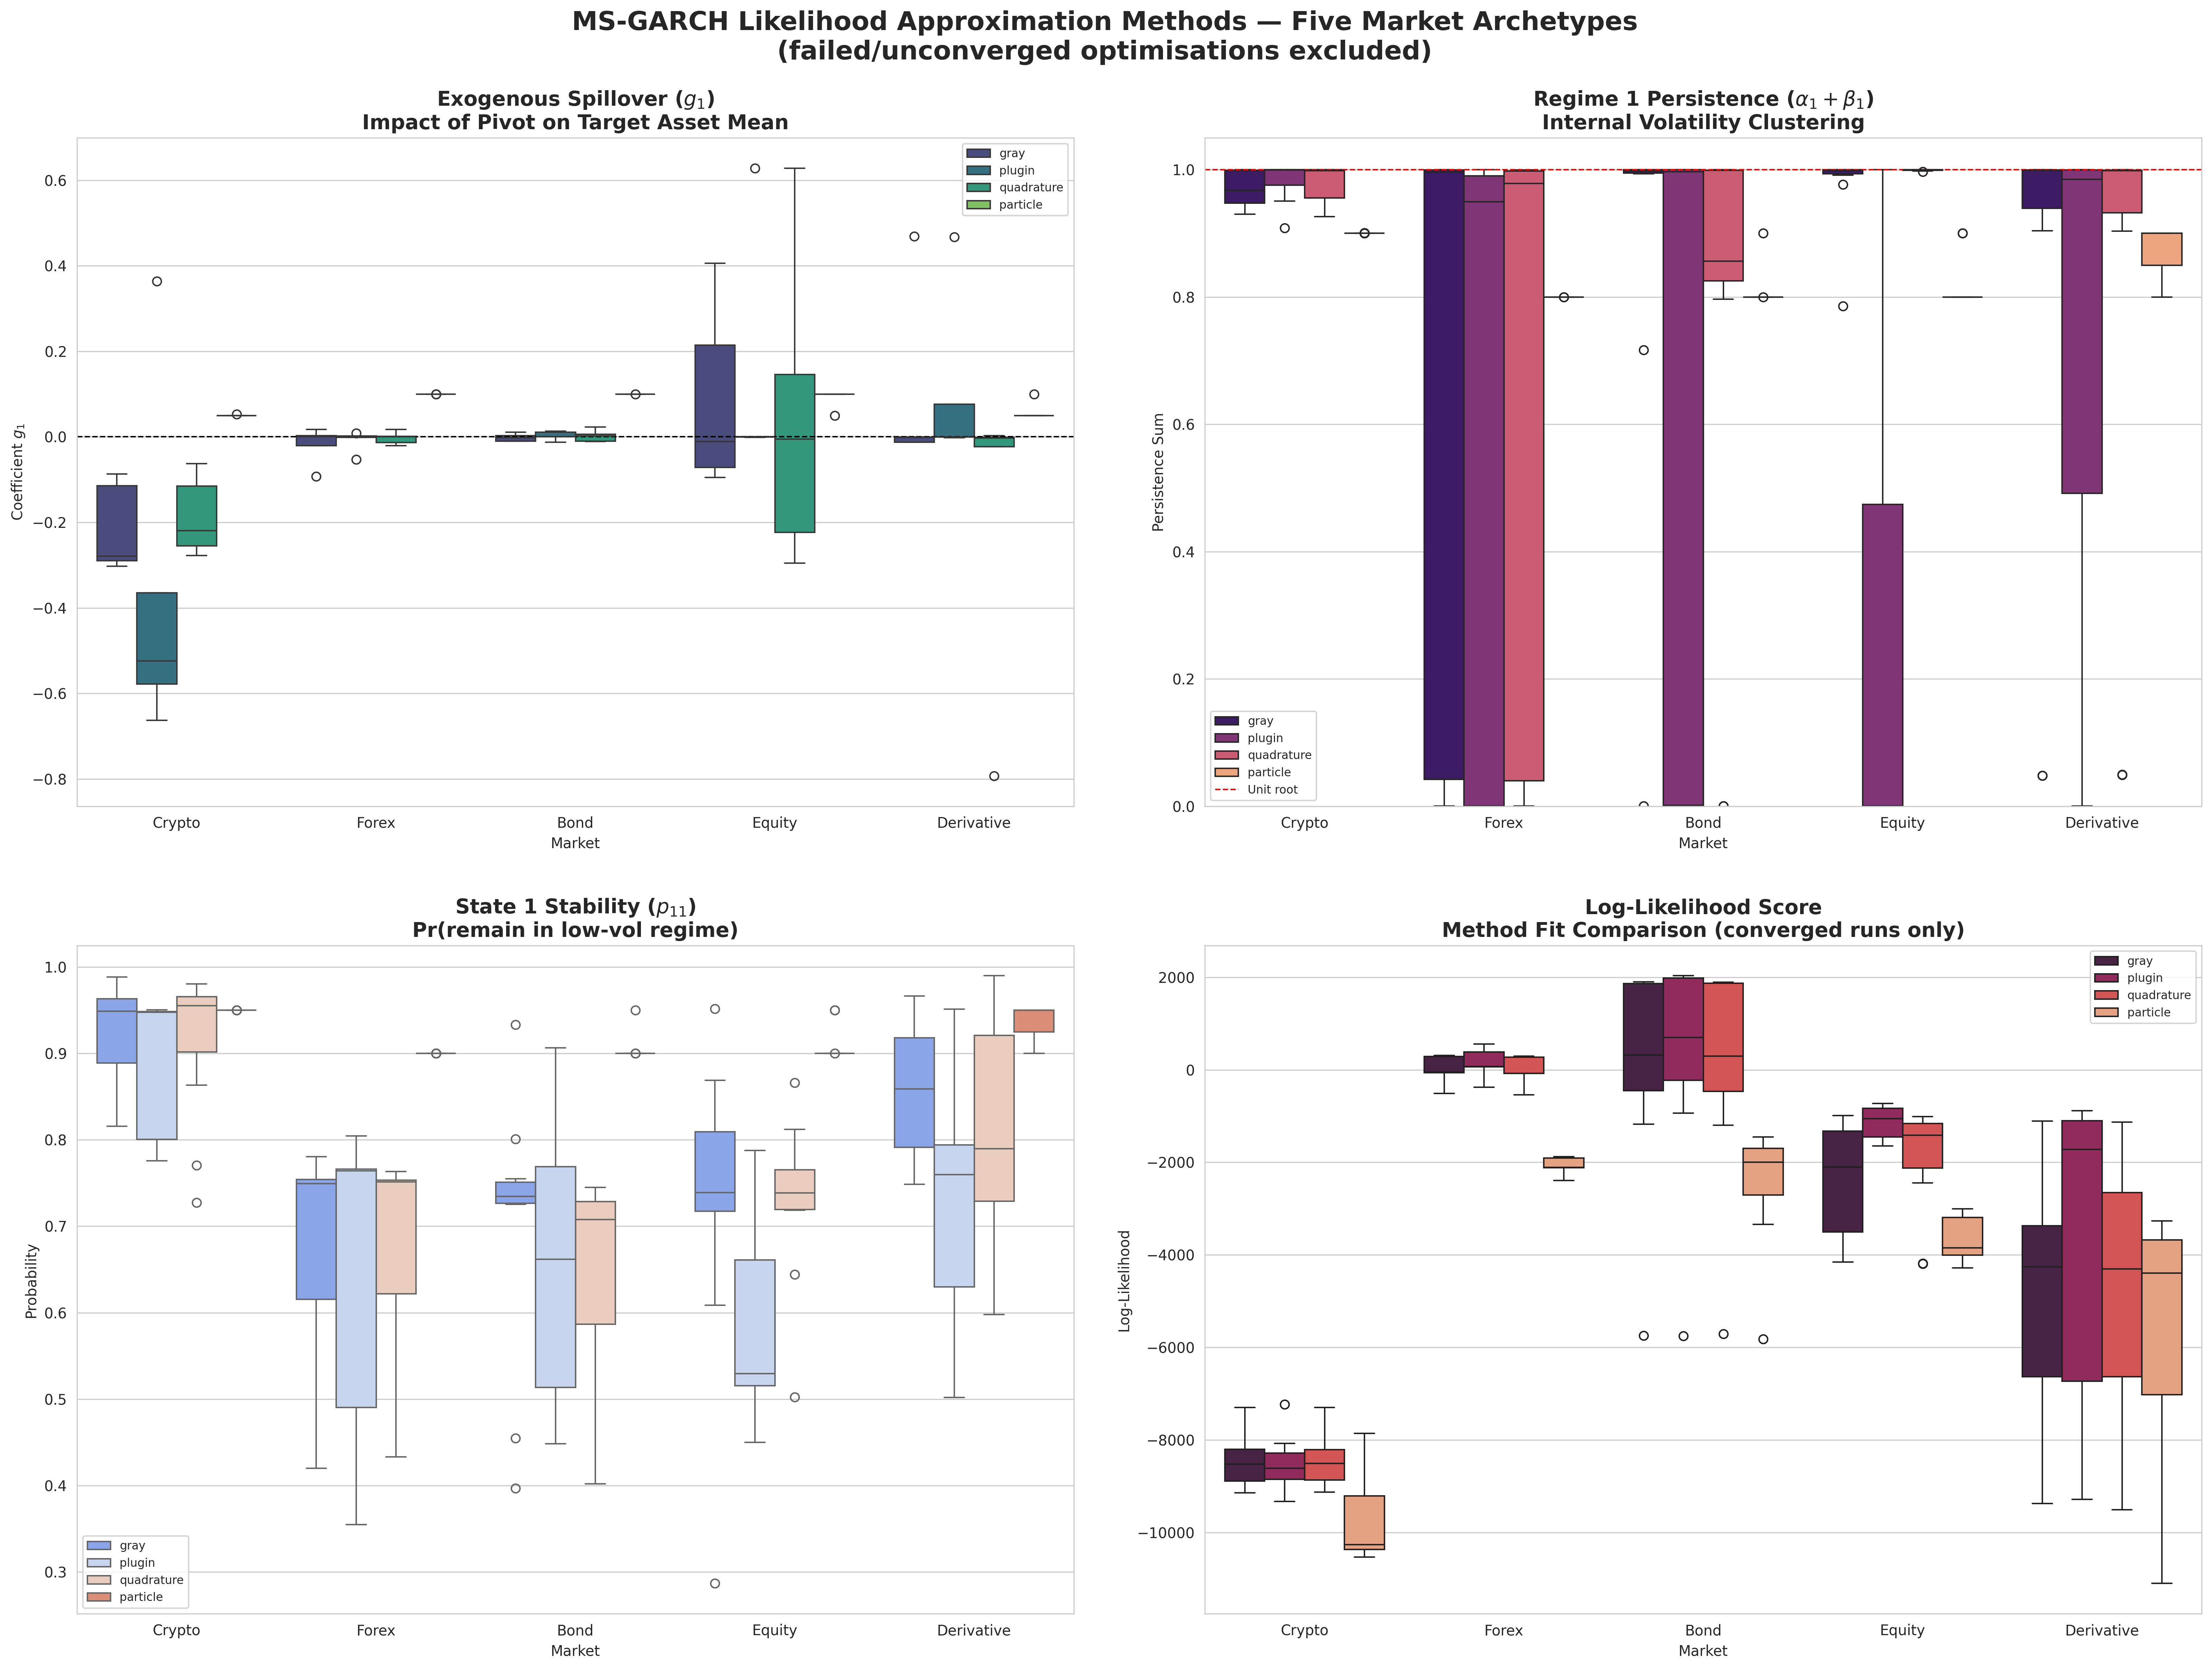
\includegraphics[width=\textwidth]{MSGARCH_Comparative_Analysis.png}
\caption{Comparative Log-Likelihood Performance of the Four Approximation Methods Across Market Archetypes. Higher values indicate superior model fit. Particle Filter results are plotted on a secondary scale for readability.}
\label{fig:comparative}
\end{figure}

Bond Market.
The bond market results demonstrated Plug-in superiority for most assets while revealing the unique estimation difficulty posed by the 10-year Treasury yield (TNX). In the baseline specification, Plug-in achieved the best log-likelihood for IEI ($2{,}031.30$ vs. Gray's $1{,}896.91$), BNDX ($1{,}992.60$ vs. Gray's $1{,}854.41$), LQD ($482.71$, non-converged, vs. Gray's $310.69$), HYG ($697.38$ vs. Quadrature's $579.36$), and TLT ($-934.93$ vs. Gray's $-1{,}173.63$). The TNX itself proved the most numerically problematic bond instrument: Gray and Plug-in both failed to converge in the baseline, and only Quadrature converged at a log-likelihood of $-5{,}708.41$, indicating fundamental difficulty for standard moment-matching and probability-weighting approaches in capturing the non-standard volatility of short-rate instruments. The Particle Filter converged for all bond assets but produced log-likelihoods thousands of units below the analytical alternatives ($-1{,}455$ to $-5{,}822$), reflecting parameter trapping. In the exogenous configuration conditioned on TNX, Plug-in retained the best log-likelihood for TLT ($-926.61$), BNDX ($1{,}965.75$), LQD ($467.55$), and HYG ($745.60$, non-converged). The TNX pivot produced modest changes in log-likelihood for most assets — IEI Gray moved from $1{,}896.91$ to $1{,}891.71$, a marginal decrease — confirming that the Treasury yield factor does not dramatically restructure bond volatility dynamics beyond what internal GARCH parameters already capture. The bond market exhibited a distinctive persistence structure: most assets showed near-zero persistence in one state ($p_{ii} \approx 0.0002$) and near-unit persistence in the other ($p_{ii} > 0.99$), consistent with a highly persistent low-volatility regime interrupted by brief high-volatility episodes. HYG was a notable exception, with non-trivial second-state persistence ($0.31$ under the Gray exogenous model), reflecting the credit-cycle sensitivity of high-yield instruments relative to investment-grade alternatives.

Derivatives Market.
The derivatives market produced the starkest divergence in approximation method performance among all five market archetypes. In the baseline, Plug-in achieved the best log-likelihood for ES=F ($-1{,}095.35$ vs. Gray's $-3{,}363.57$, a gap of over 2{,}200 units), NQ=F ($-1{,}708.53$ vs. Gray's $-4{,}168.20$, a gap exceeding 2{,}400 units), GC=F ($-884.73$ vs. Gray's $-1{,}105.49$), and CL=F ($-5{,}767.89$, non-converged, marginally superior to Quadrature's $-5{,}819.91$). For BTC=F, Gray and Quadrature converged to nearly identical results ($-7{,}441.63$ and $-7{,}441.91$) and outperformed Plug-in ($-7{,}692.15$, non-converged), suggesting that Bitcoin futures behave more like cryptocurrency assets where Gray-type approximations are better suited. The VIX index was the most pathological case in the entire 220-case study: all three analytical methods — Gray, Plug-in, and Quadrature — failed to converge in both baseline and exogenous configurations, with log-likelihoods ranging from $-9{,}248$ to $-9{,}503$. The Particle Filter was the only method to achieve formal convergence for VIX in all specifications, though its log-likelihood ($-11{,}097$ to $-11{,}098$) was substantially worse than the non-converged analytical solutions, confirming that the VIX's extreme asymmetric volatility dynamics are fundamentally intractable for all current MS-GARCH(1,1) approximation strategies. In the exogenous configuration conditioned on BTC=F, Plug-in retained its performance advantage for ES=F ($-1{,}108.91$) and NQ=F ($-1{,}717.33$). A notable anomaly appeared for CL=F: the Plug-in exogenous model reached $-3{,}123.80$ (non-converged) — dramatically better than Gray or Quadrature (both near $-5{,}823$) — suggesting a structurally different regime decomposition when Bitcoin futures are included as a conditioning variable for crude oil volatility. The VIX remained intractable for all analytical methods in the exogenous specification, continuing to confirm the fundamental numerical limitations of deterministic approximation methods for this fear-gauge instrument.

% ===========================================================
\section{Discussion}
\label{sec:discussion}
% ===========================================================

To derive a generalisable and actionable inference framework, the results are now interpreted through the lens of excess kurtosis, which serves as the primary observable indicator of distributional tail risk and likelihood surface complexity. This kurtosis-based classification organises the 30 assets irrespective of market archetype, establishing a data-driven framework for method selection that addresses the key methodological gap identified in the introduction \citep{Augustyniak2014, Ardia2018}.

Low Kurtosis ($K < 10$).
For assets with low excess kurtosis — primarily Forex pairs (EURUSD=X: $K = 4.49$; JPY=X: $K = 6.56$; AUDUSD=X: $K = 6.83$; GBPUSD=X: $K = 8.04$; CHF=X: $K = 8.14$), short-duration bond instruments (IEI: $K = 5.68$; TLT: $K = 8.12$), the gold futures (GC=F: $K = 6.58$), LTC-USD ($K = 7.94$), and BTC=F ($K = 8.21$) — the likelihood surface is comparatively well-behaved, and the Plug-in method consistently achieved the best log-likelihood optimisation across both baseline and exogenous specifications. Gray and Quadrature methods performed competitively for these assets, achieving good convergence, but were consistently outpaced by Plug-in in log-likelihood quality \citep{Gray1996, Klaassen2002}. The Particle Filter, though numerically stable, yielded inferior fit metrics by margins of two to four thousand log-likelihood units in all cases, confirming that stochastic simulation is unnecessarily costly and imprecise for assets with well-behaved return distributions \citep{Ardia2019}. The near-negligible improvement from exogenous conditioning for Forex assets — demonstrated by changes of less than two log-likelihood units upon incorporating EURUSD=X — confirmed that volatility in major currency markets is driven predominantly by internal dynamics over the study period \citep{Bollen2000}. For practitioners, Plug-in is the unambiguous first choice for low-kurtosis assets, with Gray as a convergence-guaranteed alternative and the Particle Filter categorically inadvisable.

Medium Kurtosis ($10 \le K < 20$).
The medium-kurtosis cohort includes equity indices (IXIC: $K = 12.87$; N225: $K = 17.57$; EEM: $K = 16.92$), bond ETFs (BNDX: $K = 11.68$), cryptocurrencies (ETH-USD: $K = 10.91$; XRP-USD: $K = 17.33$; BTC-USD: $K = 13.89$), and derivatives (NQ=F: $K = 10.58$; VIX: $K = 14.28$). Plug-in retained its advantage for most assets in this range, particularly for equity assets (FTSE, N225, IXIC, EEM) and most derivative instruments. The most significant divergence from the low-kurtosis pattern emerged for cryptocurrency assets under exogenous conditioning: for ETH-USD and LTC-USD conditioned on BTC-USD, Gray and Quadrature jointly achieved the best converged log-likelihoods while Plug-in produced inferior values and failed convergence more frequently, suggesting that the additional gamma parameters interacted adversely with Plug-in's probability-weighting logic in the crypto likelihood environment \citep{Augustyniak2014, Ardia2018}. Quadrature thus demonstrated its strongest comparative advantage specifically for exogenous cryptocurrency models in the medium kurtosis range. The VIX — classified as medium kurtosis at $K = 14.28$ but exhibiting uniquely asymmetric, spike-dominated volatility — was the sole instrument for which all three analytical methods failed to converge in every specification \citep{Catania2017}. The Particle Filter converged for VIX but at a log-likelihood substantially below the non-converged analytical solutions, illustrating that convergence alone does not constitute adequate model fit. For practitioners working in the medium-kurtosis range, Plug-in remains the preferred baseline estimator, with Quadrature as the preferred alternative for exogenous cryptocurrency specifications. The VIX represents a recognised estimation boundary for the standard 12-parameter MS-GARCH(1,1) framework.

High Kurtosis ($20 \le K < 50$).
High-kurtosis assets include equity ETFs (VTV: $K = 27.39$; FTSE: $K = 25.19$; GSPC: $K = 22.64$), corporate bond ETFs (LQD: $K = 36.95$; HYG: $K = 37.30$), derivatives (ES=F: $K = 20.95$; CL=F: $K = 39.31$; TNX: $K = 47.73$), and NMC-USD ($K = 29.31$). Plug-in continued to lead in likelihood maximisation for equity assets and most bond instruments, but convergence reliability became markedly more variable at these kurtosis levels: EEM Plug-in converged in the baseline but Gray failed; N225 Gray converged in the baseline but deteriorated dramatically in the exogenous model; and multiple Quadrature results failed convergence for NQ=F and IXIC. The large Plug-in advantages for ES=F and NQ=F — exceeding 2{,}200 and 2{,}400 log-likelihood units over Gray and Quadrature, respectively — represent the most extreme method-performance divergences in the entire study, indicating that the multi-modal likelihood surfaces generated by high-kurtosis financial futures are particularly poorly navigated by moment-matching procedures. For BTC=F and TNX, however, Gray and Quadrature proved more reliable than Plug-in in achieving convergent solutions with competitive likelihoods, suggesting that for specific high-kurtosis instruments with structural regularities different from equity-index futures, moment-matching methods retain practical utility \citep{Haas2004}. The Particle Filter remained the weakest performer in log-likelihood across all high-kurtosis assets, though it achieved broad convergence. For practitioners in the high-kurtosis range, Plug-in should be attempted first with mandatory convergence verification, with Gray or Quadrature employed as convergence-reliable fallbacks. The Particle Filter is appropriate only as a last resort when all analytical methods fail entirely.

Extreme Kurtosis ($K \ge 50$).
Only two assets in the corpus fall in the extreme-kurtosis category: DOGE-USD ($K = 98.51$) and EURGBP=X ($K = 248.50$). Contrary to conventional expectations in the literature, which suggest that simulation-based methods should become preferable at very high kurtosis levels, the Particle Filter did not emerge as the superior method for either asset. For DOGE-USD, Plug-in achieved the best baseline log-likelihood ($-8{,}613.45$, non-converged) while the Particle Filter converged to a markedly inferior $-10{,}260.15$ — a deficit of over 1{,}600 units. For EURGBP=X, Plug-in fully converged to a log-likelihood of $557.11$ while the Particle Filter converged to $-1{,}878.74$ — a deficit approaching 2{,}500 units — representing the largest absolute gap between an analytical and simulation-based method in the entire study. These findings indicate that even at kurtosis levels exceeding 50 to 248, the Particle Filter serves only as a last-resort fallback for obtaining any convergent solution when all analytical methods fail completely, not as the preferred estimator for heavy-tailed data \citep{Doucet2001, Pitt1999}. For practitioners encountering extreme-kurtosis assets, Plug-in should still be attempted first; the Particle Filter should be reserved exclusively for situations where all analytical methods fail to produce any solution, with expectations appropriately adjusted regarding the quality of Particle Filter parameter estimates.

Summary Framework.
Table~\ref{tab:framework} synthesises the kurtosis-based method-selection recommendations emerging from the empirical analysis. The overarching pattern is that the Plug-in approximation is the dominant likelihood optimiser across all four kurtosis classes, with its advantage growing most pronounced for high-kurtosis equity-index futures. The Particle Filter is consistently the weakest likelihood optimiser and should be used only when all analytical alternatives fail completely. Quadrature demonstrates its strongest relative advantage for medium-kurtosis cryptocurrency assets in the exogenous specification. Exogenous conditioning improves model fit selectively — most consistently for bond and equity markets — and should not be assumed universally beneficial without prior empirical validation.

\begin{table}[ht]
\centering
\small
\caption{Kurtosis-Based Method-Selection Framework for MS-GARCH Estimation}
\label{tab:framework}
\begin{tabular}{p{2.2cm} p{2.8cm} p{2.8cm}}
\toprule
\textbf{Kurtosis Class} & \textbf{Preferred Method} & \textbf{Fallback / Notes} \\
\midrule
Low ($K < 10$) & Plug-in (baseline \& exog.) & Gray for convergence guarantee; Particle Filter inadvisable \\[4pt]
Medium ($10\!\le\! K < 20$) & Plug-in (baseline); Quadrature (exog. crypto) & Gray for convergence; VIX intractable for all analytical methods \\[4pt]
High ($20\!\le\! K < 50$) & Plug-in (verify convergence) & Gray / Quadrature as fallback; Particle Filter last resort \\[4pt]
Extreme ($K \ge 50$) & Plug-in (attempt first) & Particle Filter only if all analytical methods yield no solution \\
\bottomrule
\end{tabular}
\end{table}

% ===========================================================
\section{Conclusion}
\label{sec:conclusion}
% ===========================================================

This study undertook the first large-scale, controlled comparative evaluation of four MS-GARCH likelihood approximation methods — Gray's collapsing procedure, Plug-in, Gaussian Quadrature, and Particle Filtering — across thirty financial assets spanning five market archetypes and 220 experimental cases. The central finding is unequivocal: the choice of likelihood approximation method materially affects estimation outcomes, and this choice should be grounded in the observable statistical properties of the data rather than software convention or disciplinary tradition.

The Plug-in method emerged as the dominant approximation across all kurtosis classes and all five market archetypes in terms of log-likelihood maximisation. For low-kurtosis assets, Plug-in consistently outperformed all alternatives. For high-kurtosis equity-index futures (ES=F, NQ=F), the Plug-in advantage over Gray and Quadrature exceeded 2{,}000 to 2{,}400 log-likelihood units — differences with significant practical implications for model comparison, inference, and risk management applications. The Particle Filter was, without exception, the weakest likelihood optimiser across all kurtosis classes and market archetypes, systematically underperforming by two to four thousand units while exhibiting parameter degeneracy near initialisation values. The only context in which the Particle Filter provided value was as a convergence fallback for the VIX and for situations in which all analytical methods failed entirely. Quadrature's strongest relative advantage appeared specifically for cryptocurrency assets in exogenous specifications within the medium-kurtosis range, where its superior convergence stability relative to Plug-in made it the preferred convergence-adjusted choice.

Exogenous conditioning produced selective rather than uniform improvements in model fit. Bond market assets benefited most consistently from the Treasury yield pivot. Forex assets showed negligible improvement from the EURUSD=X factor, confirming the idiosyncratic nature of developed-market currency volatility. The VIX represents a fundamental estimation challenge: no analytical MS-GARCH approximation method converged for this instrument under the adopted 12-parameter specification, pointing to the need for extended model frameworks — potentially asymmetric or three-regime specifications — to accommodate the non-standard dynamics of fear-gauge instruments.

Practitioners are advised to adopt the kurtosis-informed framework summarised in Table~\ref{tab:framework}: calculate excess kurtosis before selecting an approximation method; default to Plug-in for most asset classes with Gray or Quadrature as convergence-reliable fallbacks; avoid the Particle Filter except as a last resort; and validate exogenous conditioning variables empirically before including them as standard model components. Researchers are encouraged to report convergence status alongside parameter estimates, document the approximation method employed, and perform at minimum a two-method robustness comparison when publishing MS-GARCH results.

\section*{Acknowledgements}

The authors acknowledge the Federal University of Technology, Akure (FUTA) for institutional support. Computational work was performed using open-source Python libraries including \texttt{scipy}, \texttt{numpy}, \texttt{yfinance}, and a custom C++/Cython MS-GARCH estimation engine.

\section*{Data Availability}

All financial data were retrieved from Yahoo Finance via the \texttt{yfinance} Python library (freely available). The complete CSV results database, parameter estimates, visualisations, and estimation code are available at the project GitHub repository.

% ---- REFERENCES ----
\bibliography{references}

\end{document}
